\chapter{Evaluation}
\label{sec:evaluation}
This chapter describes experiments that I conducted to evaluate the effectiveness of the proposed method. Specifically, I evaluated the heart rate acquired by a smartwatch when an arbitrary target heart rate was given. I then observed the error between the target heart rate and the heart rate obtained by the smartwatch and investigated the effects of various smartwatches and displays.

% 4.1
\section{Evaluation Environment}
I used five smartwatches for the evaluation experiment: the TicWatch Pro WF12106, Puma Smartwatch PT9100, Apple Watch Series 3 and Series 5, and SMART R F-18. I also used four different displays: the display of the Lenovo Legion 7 15IMH05 laptop (display A); two 3.5-inch displays developed for Raspberry Pi by Elecrow and Osoyoo (displays B and C, respectively); and a lightweight flexible display \cite{flexible_display} that Kawahara et al. constructed (display D). Figure \ref{fig:smartwatches} shows all the smartwatches and displays that I used, and Figure \ref{fig:flexible} shows the details of display D.

\begin{figure}[!t]
  \centering
  \includegraphics[width=1\linewidth]{figures/smartwatches.eps}
  \caption{Smartwatches and displays used in the experiment.}
  \label{fig:smartwatches}
\end{figure}

\begin{figure}[!t]
  \centering
  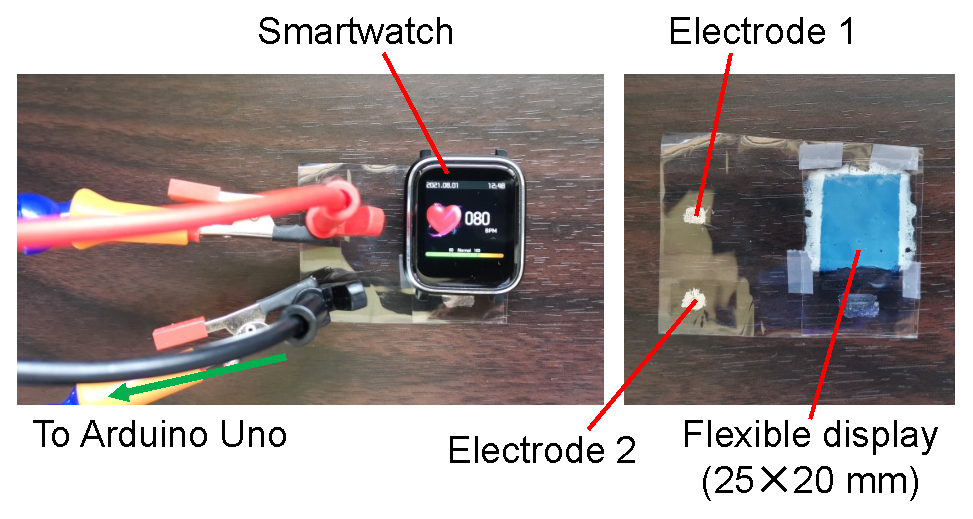
\includegraphics[width=1\linewidth]{figures/flexible.eps}
  \caption{Illustration of the flexible display (display D).}
  \label{fig:flexible}
\end{figure}


% 4.2
\section{Display Drawing Program Implementations}
The four displays used in the evaluation experiment had different connection methods to the computer. Display A was a laptop display, and commercial displays B and C could use an HDMI connection. In contrast, display D required drawing on the screen by controlling the voltage applied to the display's electrodes. In this chapter, I explain the display drawing programs that I implemented to control each display.

% 4.2.1
\subsection{Displays A, B, and C}
Displays A, B, and C were all recognized by the computer as regular displays. The $Colors$ data was represented in grayscale, a type of computer color representation that uses 256 levels (0--255) to represent shades of color from black to white (i.e., smaller values represent darker shades). Each array element $Colors[i]~(i=0,\dots,L)$ was generated by the following equation:
\begin{equation}
  Colors[i]=\min\left(\sin\left(\frac{2\pi i}{L}\right)+1,1\right)*SCALE+BASE,
\end{equation}
where the values of $L$, $SCALE$, and $BASE$ were heuristically determined in advance for each display-smartwatch combination.\par

For example, if $L=19$, $SCALE=30$, and $BASE=225$, then $Colors$ was obtained as the following sequence of numbers:
\begin{equation*}
  \begin{split}
    Colors = [255, 255, 255, 255, 255, 255, 255, 255, 255, 255,\\250, 240, 232, 227, 225, 225, 229, 236, 245, 255]
  \end{split}
\end{equation*}
Figure \ref{fig:colors_wave} shows a plot of this particular $Colors$ array.\par

A program to change the brightness of displays A, B, and C was implemented with Python and Processing. Processing\footnote{\url{https://processing.org}} is a Java-based programming language that is excellent for visual expression and is used to create electronic art and visual designs. Here, the Processing component receives the target heart rate from the Python component, and it uses the \texttt{background} method to draw the appropriate grayscale background color on the display.

\begin{figure}[!t]
  \centering
  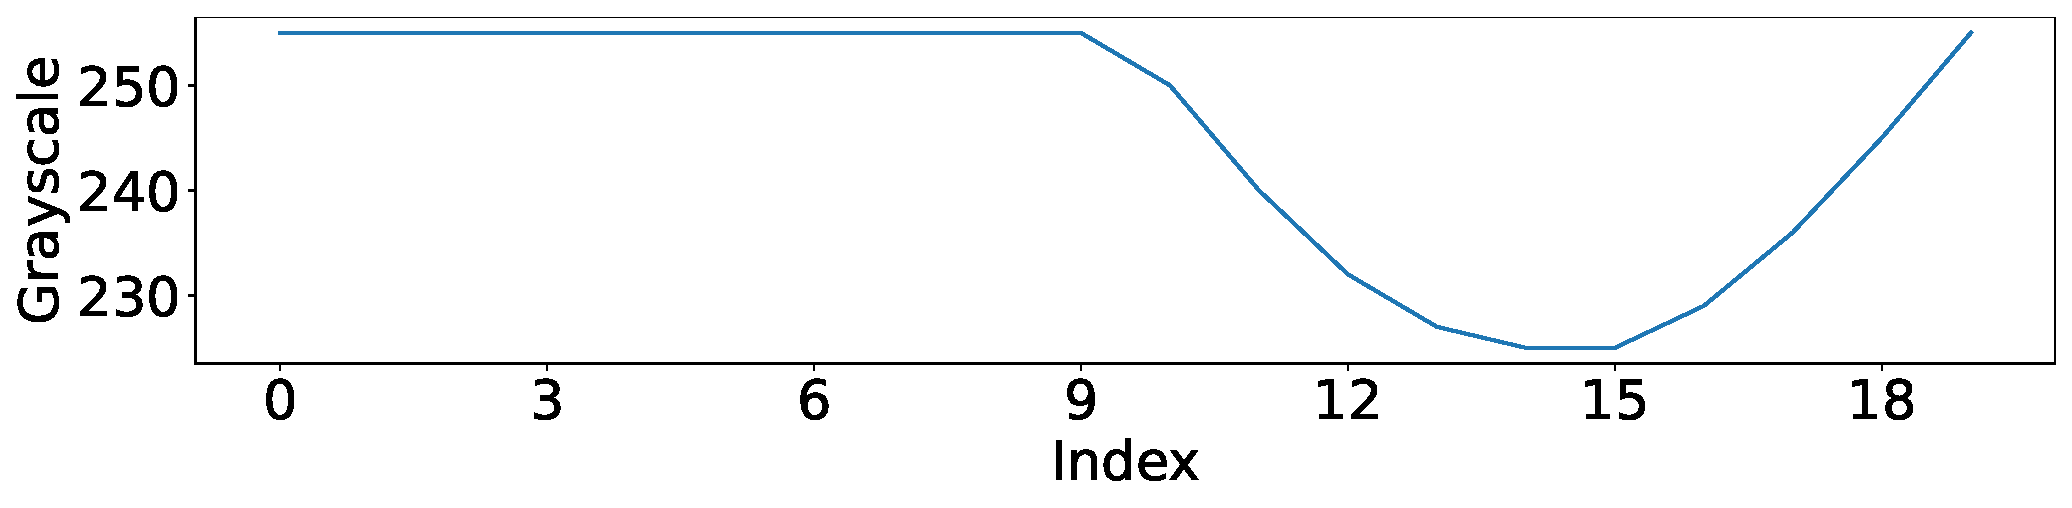
\includegraphics[width=1\linewidth]{figures/colors_wave.eps}
  \caption{Example plot of light and dark changes in the display for the smartwatch to detect a single pulse peak.}
  \label{fig:colors_wave}
\end{figure}

% 4.2.2
\subsection{Display D}
Display D was made of a flexible film that could fit on curved areas like an arm or the back of a smartwatch, but it did not have HDMI capability. Instead, it was made to blink by switching the potential direction applied to its terminals. The display color became darker when a higher voltage was applied to electrode 1 and lighter when a higher voltage was applied to electrode 2.\par

As a result of a heuristic search in a preliminary study, $Colors$ was determined to be the following sequence of colors for display D:
\begin{equation*}
  \begin{split}
    Colors = [BLACK, WHITE].
  \end{split}
\end{equation*}
For $BLACK$, I set the voltage of electrode 1 to 2 V and that of electrode 2 to 0 V; for $WHITE$, I set the voltage of electrode 1 to 0 V and that of electrode 2 to 2 V. Figure \ref{fig:colors_flexible} shows how the voltage changed when the pattern in $Colors$ was repeated twice.\par

For display D, I implemented a display drawing program by using the Arduino Uno R3 microcomputer, which could control the output voltage by pulse-width modulation (PWM). After receiving the target heart rate from the Python component running on a connected computer, the Arduino changed the voltage to the display.

\begin{figure}[!t]
  \centering
  \includegraphics[width=1\linewidth]{figures/voltage_wave.eps}
  \caption{Voltage changes when the pattern in $Colors$ was repeated twice.}
  \label{fig:colors_flexible}
\end{figure}


% 4.3
\section{Data Acquisition}
Depending on the installed operating system (OS), the five smartwatches had different ways of acquiring the heart rate. In this section, I describe how the heart rate was acquired for each OS.

% 4.3.1
\subsection{Wear OS}
The TicWatch Pro WF12106 and the Puma Smartwatch PT9100 both use Wear OS by Google\footnote{\url{https://wearos.google.com}}, an OS that was designed for smartwatches and is based on Android. I used Android Studio\footnote{\url{https://developer.android.com/studio}} to implement the control application, which is illustrated in Figure \ref{fig:app}.\par

When the application is started, it displays the screen shown in (1). Acquisition of the sensor value starts automatically, and when the value changes, it is displayed as shown in (2). ``Heart'' indicates the value from the heart rate sensor, and ``Pulse'' indicates the value from the PPG sensor. Data recording is begun by tapping the ``RECORD'' button. A 60-s calibration then starts as shown in (3). This calibration waits for the sensor value to stabilize, and the wearing position of the smartwatch can be adjusted during this period. When the 60-s calibration is complete, sensor data is acquired for 60 s as shown in (4) and stored in a variable. At the end of the data acquisition period, the data stored in the variable is saved to the smartwatch in CSV format, and a message indicating the completion of data acquisition is displayed as shown in (5). The smartwatch is equipped with a variety of sensors, and the data is accessed by specifying the sensor number during application development\footnote{\url{https://developer.android.com/reference/android/hardware/Sensor}} (e.g., sensor number 21 and 65572 for the heart rate sensor and the PPG sensor in this application). The rate of ``SENSOR\_DELAY\_UI'' events was used to set a sampling rate that was suitable for implementing the user interface\footnote{\url{https://developer.android.com/reference/android/hardware/SensorManager}}.\par

In the evaluation experiment, data acquisition was started by placing the smartwatch on the display, entering the target heart rate into the standard input of the display drawing program, and tapping the ``RECORD'' button in the smartwatch application. After 120 s, including the 60-s calibration, the data acquisition was complete. The sampling rate for heart rate data acquisition was approximately 1 Hz. As shown in Figure \ref{fig:calculating_wearos}, the time average of 60 s of data (excluding the calibration period) was calculated, and the result was obtained as the heart rate.

\begin{figure}[!t]
  \centering
  \includegraphics[width=1\linewidth]{figures/app.eps}
  \caption{Details of the control application implemented for the Wear OS smartwatches.}
  \label{fig:app}
\end{figure}

\begin{figure}[!t]
  \centering
  \begin{minipage}[t]{1\linewidth}
    \centering
    \includegraphics[width=1\linewidth]{figures/calculating_wearos.eps}
    \subcaption{Wear OS smartwatches}
    \small The time average of 60 s of data, excluding the 60 s of calibration time, was calculated as the heart rate result.
    \label{fig:calculating_wearos}
    \vspace{10pt}
  \end{minipage}
  \begin{minipage}[t]{1\linewidth}
    \centering
    \includegraphics[width=1\linewidth]{figures/calculating_watchos.eps}
    \subcaption{watchOS smartwatches}
    \small The first 30 s of data was excluded as calibration time, and the time average of the following 60 s of data was calculated as the heart rate result.
    \label{fig:calculating_watchos}
    \vspace{10pt}
  \end{minipage}
  \begin{minipage}[t]{1\linewidth}
    \centering
    \includegraphics[width=1\linewidth]{figures/calculating_smartos.eps}
    \subcaption{SMART OS smartwatch}
    \small The heart rate displayed in the app was recorded manually as the heart rate result.
    \label{fig:calculating_smartos}
  \end{minipage}
  \caption{Heart rate calculations for the smartwatches in the evaluation experiment.}
  \label{fig:calculating_heart_rate}
\end{figure}

% 4.3.2
\subsection{watchOS}
The Apple Watch Series 3 and Series 5 come standard with Apple's Heart Rate app that measures the heart rate\footnote{\url{https://support.apple.com/en-us/HT204666}}. The collected heart rate data can be output as numerical data in XML format by using the iPhone Health app when paired with the Apple Watch\footnote{\url{https://support.apple.com/guide/iphone/share-health-and-fitness-data-iph27f6325b2/ios}}.\par

In the evaluation experiment, data acquisition was started by placing the smartwatch on the display, entering the target heart rate into the standard input of the display drawing program, and launching the Heart Rate app. After a period of time, the Apple Watch display automatically turned off, and the data acquisition was complete. The data acquisition time was not configurable, but I found a maximum time of approximately 160 s. The sampling rate was not publicly accessible, and the amount of data acquired in a single data acquisition trial varied. As shown in Figure \ref{fig:calculating_watchos}, the first 30 s of data was excluded as calibration time, and the time average of the following 60 s of data was calculated as the result for the heart rate. However, when no data was acquired after the calibration time, the last acquired data was used as the heart rate.

% 4.3.3
\subsection{SMART OS}
The SMART R F-18 is equipped with a proprietary OS developed by the manufacturer, and I refer to it here as ``SMART OS.'' Heart rate data collected by this smartwatch can be viewed with the WearHealth app for Android\footnote{\url{https://play.google.com/store/apps/details?id=com.zjw.wearhealth}} and iPhone\footnote{\url{https://apps.apple.com/us/app/wearhealth/id1265052549}}.\par

In the evaluation experiment, data acquisition was started by placing the smartwatch on the display, entering the target heart rate into the standard input of the display drawing program, and controlling the smartwatch from the WearHealth app on the smartphone. After 30 s, the data acquisition was complete, and the resulting heart rate was displayed in the app. The sampling rate and the algorithm to determine the resulting heart rate were not publicly accessible for the SMART R F-18. As shown in Figure \ref{fig:calculating_smartos}, the heart rate result shown in the app was recorded manually.


% 4.4
\section{Results and Discussion}
To obtain the correct heart rate, an acrylic plate of a certain thickness was placed between the display and the smartwatch in some display-smartwatch combinations. Table \ref{tab:acrylic_plate} lists these combinations and the thicknesses of the acrylic plate, with a blank cell indicating that the plate was not used.\par

The error of the measured heart rate was calculated by subtracting the target heart rate from it. The target heart rate was tested at intervals of 5 bpm from 60 to 100 bpm, which is the resting heart rate range for adults\footnote{\url{https://www.heart.org/en/healthy-living/fitness/fitness-basics/target-heart-rates}}. Table \ref{tab:result} lists the results of the evaluation experiment, which were averaged over three sets of measurements. The results were rounded to the first decimal place. A zero means that the measured heart rate was the same as the target heart rate, and a negative value means that the measured heart rate was smaller. An $NaN$ entry indicates that the heart rate measurement failed.\par

In addition, Table \ref{tab:result_expansion} lists the results of a separate experiment using display D with target heart rates set of 40--55 bpm (heart rate during sleep) and 105--200 bpm (heart rate during exercise).

\begin{table*}[!t]
  \centering
  \caption{Thickness of the acrylic plate placed between the display and the smartwatch.}
  \begin{tabular}{cccc|cccc}
    \toprule
    \multicolumn{4}{c|}{TicWatch Pro}&\multicolumn{4}{c}{Puma} \\
    A & B & C & D & A & B & C & D \\
    \midrule
    -- & 2 mm & -- & 5 mm & -- & -- & -- & 2 mm \\
    \bottomrule
  \end{tabular}
  \begin{tabular}{cccc|cccc|cccc}
    \toprule
    \multicolumn{4}{c|}{Series 3}&\multicolumn{4}{c|}{Series 5}&\multicolumn{4}{c}{SMART R} \\
    A & B & C & D & A & B & C & D & A & B & C & D \\
    \midrule
    -- & -- & -- & -- & -- & 2 mm & -- & -- & 2 mm & -- & -- & -- \\
    \bottomrule
  \end{tabular}
  \label{tab:acrylic_plate}
\end{table*}

\begin{table*}[!t]
  \small
  \centering
  \caption{Error in the resting heart rate obtained by the TicWatch Pro, Puma Smartwatch, Apple Watch Series 3, Apple Watch Series 5, and SMART R (display A: Lenovo Legion 7; B: 3.5-inch Elecrow; C: 3.5-inch Osoyoo; D: flexible display).}
  \begin{tabular}{c|cccc|cccc}
    \toprule
    &\multicolumn{4}{c|}{TicWatch Pro}&\multicolumn{4}{c}{Puma} \\
    $H_{target}$ & A & B & C & D & A & B & C & D \\
    \midrule
    $60$ & $-1.7$ & $-1.4$ & $-1.4$ & $-2.0$ & $-1.7$ & $-1.4$ & $-1.4$ & $-0.8$ \\
    $65$ & $-1.8$ & $-1.4$ & $-1.3$ & $-2.5$ & $-1.8$ & $-1.4$ & $-1.3$ & $-1.8$ \\
    $70$ & $-1.8$ & $-2.1$ & $-1.2$ & $-0.4$ & $-1.8$ & $-2.1$ & $-1.2$ & $-0.9$ \\
    $75$ & $-2.2$ & $-1.6$ & $-1.5$ & $-0.1$ & $-2.2$ & $-1.6$ & $-1.5$ & $-1.2$ \\
    $80$ & $-2.0$ & $-1.5$ & $-1.1$ & $0.6$ & $-2.0$ & $-1.5$ & $-1.1$ & $0.0$ \\
    $85$ & $-1.8$ & $-1.5$ & $-1.6$ & $0.5$ & $-1.8$ & $-1.5$ & $-1.6$ & $0.3$ \\
    $90$ & $-2.0$ & $-1.7$ & $-1.0$ & $-0.4$ & $-2.0$ & $-1.7$ & $-1.0$ & $-0.5$ \\
    $95$ & $-2.0$ & $-1.2$ & $-1.1$ & $0.0$ & $-2.0$ & $-1.2$ & $-1.1$ & $-1.2$ \\
    $100$ & $-1.9$ & $-1.5$ & $-1.4$ & $-1.0$ & $-1.9$ & $-1.5$ & $-1.4$ & $-1.2$ \\
    \midrule
    Average & $-1.9$ & $-1.5$ & $-1.3$ & $-0.6$ & $-1.9$ & $-1.5$ & $-1.3$ & $-0.8$ \\
    \bottomrule
  \end{tabular}
  \begin{tabular}{c|cccc|cccc}
    \toprule
    &\multicolumn{4}{c|}{Series 3}&\multicolumn{4}{c}{Series 5} \\
    $H_{target}$ & A & B & C & D & A & B & C & D \\
    \midrule
    $60$ & $0.4$ & $1.0$ & $-0.2$ & $NaN$ & $58.2$ & $0.1$ & $-0.1$ & $0.0$ \\
    $65$ & $0.6$ & $0.1$ & $-0.1$ & $NaN$ & $16.1$ & $-0.4$ & $0.1$ & $0.0$ \\
    $70$ & $0.1$ & $2.0$ & $0.0$ & $NaN$ & $1.6$ & $2.4$ & $0.1$ & $0.0$ \\
    $75$ & $0.0$ & $2.8$ & $-0.6$ & $NaN$ & $0.8$ & $0.1$ & $-0.2$ & $-0.1$ \\
    $80$ & $-0.5$ & $1.0$ & $-0.5$ & $NaN$ & $1.2$ & $0.9$ & $-0.4$ & $-0.5$ \\
    $85$ & $-5.4$ & $-0.7$ & $-0.6$ & $NaN$ & $-0.6$ & $-1.0$ & $-0.9$ & $0.0$ \\
    $90$ & $-0.6$ & $-1.3$ & $-0.6$ & $NaN$ & $4.3$ & $-1.0$ & $-0.9$ & $0.0$ \\
    $95$ & $-1.5$ & $-0.5$ & $-1.0$ & $NaN$ & $-0.1$ & $-0.3$ & $-1.1$ & $0.0$ \\
    $100$ & $-0.7$ & $-1.1$ & $-0.7$ & $NaN$ & $-0.2$ & $-7.3$ & $-0.8$ & $-32.7$ \\
    \midrule
    Average & $-0.8$ & $0.4$ & $-0.5$ & $NaN$ & $9.0$ & $-0.7$ & $-0.5$ & $-3.7$ \\
    \bottomrule
  \end{tabular}
  \begin{tabular}{c|cccc}
    \toprule
    &\multicolumn{4}{c}{SMART R} \\
    $H_{target}$ & A & B & C & D \\
    \midrule
    $60$ & $-1.7$ & $-1.0$ & $-1.7$ & $-0.7$ \\
    $65$ & $-1.7$ & $-1.0$ & $-0.7$ & $-0.7$ \\
    $70$ & $-1.0$ & $-1.3$ & $-1.3$ & $-0.7$ \\
    $75$ & $-2.0$ & $-2.3$ & $-2.0$ & $-0.7$ \\
    $80$ & $-2.0$ & $-2.0$ & $-1.0$ & $-1.0$ \\
    $85$ & $-2.0$ & $-2.0$ & $-1.7$ & $-0.7$ \\
    $90$ & $-3.3$ & $-2.3$ & $-1.7$ & $-1.0$ \\
    $95$ & $-2.7$ & $-2.0$ & $-2.0$ & $-0.3$ \\
    $100$ & $-2.7$ & $-2.3$ & $-2.7$ & $-1.0$ \\
    \midrule
    Average & $-2.1$ & $-1.8$ & $-1.6$ & $-0.7$ \\
    \bottomrule
  \end{tabular}
  \label{tab:result}
\end{table*}

\begin{table*}[!t]
  \centering
  \caption{Error in the heart rate during sleep or exercise obtained by the TicWatch Pro, Puma Smartwatch, Apple Watch Series 3, Apple Watch Series 5, and SMART R with display D (the flexible display).}
  \begin{tabular}{c|c|c|c|c|c}
    \toprule
    & TicWatch Pro & Puma & Series 3 & Series 5 & SMART R \\
    $H_{target}$ & D & D & D & D & D \\
    \midrule
    $40$ & $0.0$ & $0.0$ & $NaN$ & $3.1$ & $23.7$ \\
    $45$ & $-1.2$ & $-1.0$ & $NaN$ & $0.1$ & $31.7$ \\
    $50$ & $-1.7$ & $-0.8$ & $NaN$ & $0.0$ & $0.3$ \\
    $55$ & $-0.7$ & $-0.7$ & $NaN$ & $0.0$ & $0.0$ \\
    \vdots & \vdots & \vdots & \vdots & \vdots & \vdots \\
    $105$ & $-0.2$ & $0.0$ & $NaN$ & $-34.3$ & $0.0$ \\
    $110$ & $-0.2$ & $0.0$ & $NaN$ & $-0.2$ & $-0.3$ \\
    $115$ & $-0.2$ & $0.3$ & $NaN$ & $-39.3$ & $-0.3$ \\
    $120$ & $-0.3$ & $-0.7$ & $NaN$ & $-41.5$ & $-0.7$ \\
    $125$ & $-0.8$ & $0.0$ & $NaN$ & $-0.7$ & $-0.3$ \\
    $130$ & $0.9$ & $0.3$ & $NaN$ & $-41.9$ & $0.0$ \\
    $135$ & $0.0$ & $-0.8$ & $NaN$ & $-41.7$ & $-0.3$ \\
    $140$ & $0.2$ & $-0.3$ & $NaN$ & $-70.7$ & $0.0$ \\
    $145$ & $0.7$ & $-0.2$ & $NaN$ & $-40.2$ & $0.3$ \\
    $150$ & $-0.1$ & $-0.3$ & $NaN$ & $-0.6$ & $-0.3$ \\
    $155$ & $0.5$ & $0.0$ & $NaN$ & $0.1$ & $0.0$ \\
    $160$ & $0.6$ & $0.0$ & $NaN$ & $0.0$ & $-0.3$ \\
    $165$ & $1.7$ & $1.3$ & $NaN$ & $0.0$ & $0.7$ \\
    $170$ & $0.0$ & $0.7$ & $NaN$ & $-94.4$ & $0.0$ \\
    $175$ & $0.3$ & $0.0$ & $NaN$ & $-50.6$ & $-0.7$ \\
    $180$ & $0.3$ & $0.6$ & $NaN$ & $-63.0$ & $0.0$ \\
    $185$ & $1.0$ & $-0.4$ & $NaN$ & $-0.3$ & $0.3$ \\
    $190$ & $1.4$ & $-0.2$ & $NaN$ & $-86.8$ & $0.3$ \\
    $195$ & $0.3$ & $1.7$ & $NaN$ & $-83.4$ & $0.3$ \\
    $200$ & $0.6$ & $0.0$ & $NaN$ & $-103.0$ & $0.0$ \\
    \bottomrule
  \end{tabular}
  \label{tab:result_expansion}
\end{table*}

% 4.4.1
\subsection{Wear OS Smartwatches}
The results showed that the heart rate could be input to the smartwatch within an error of less than $3$ bpm. For both Wear OS smartwatches, the average error was progressively smaller for displays A, B, C, and D, in that order. This suggests that differences in performance, such as the display brightness and refresh rate, may affect the generated heart rate. As seen in Table \ref{tab:result_expansion}, even when the target heart rate was set to 40--55 or 105--200 bpm, the heart rate could be input to the smartwatch within a small error.

% 4.4.2
\subsection{watchOS Smartwatches}
The results showed that display C enabled the heart rate to be input to the Apple Watches within an error of $-1.1$ to $0.1$ bpm. On the other hand, with displays A and B, I could not obtain the correct heart rate under certain conditions. In particular, the correct heart rate was not obtained even once with a target heart rate of 60 bpm and the combination of the Apple Watch Series 5 and display A.\par

When the target heart rate was set to 40--55 and 105--200 bpm, correct values were obtained for some target heart rates with the Apple Watch Series 5. When the target heart rate was set above 100 bpm, the obtained rate was very small compared to the target rate. It is possible that the Apple Watch algorithm recognized large target heart rates as incorrect and calibrated them to the heart rates during rest.\par

The combination of the Apple Watch Series 3 and display D failed to measure the heart rate regardless of the target. Because a PPG sensor uses a photoreflector, it is easily affected by light, and depending on the condition of the wearable device's placement, pulse data cannot always be acquired correctly. Whether a smartwatch can recognize a generated pulse wave is thought to depend on the shape of the device's PPG sensor. The acrylic plates that I used in this thesis could not help the performance of the Apple Watch Series 3, but it is possible that pulse data could be successfully recognized by using a plate with a different material and thickness.

% 4.4.3
\subsection{SMART OS Smartwatch}
Finally, the results showed that the heart rate could almost always be input to this smartwatch within an error of less than $3$ bpm. With display D, in particular, it could be obtained within an error of less than $1$ bpm.\par

When the target heart rate was set to 40--55 and 105--200 bpm, the heart rate could be input to the smartwatch with a very small error in many cases; for target rates below 50 bpm, however, the heart rate could not be input correctly. This is thought to be due to a performance limitation of the smartwatch's PPG sensor.
